% Options for packages loaded elsewhere
\PassOptionsToPackage{unicode}{hyperref}
\PassOptionsToPackage{hyphens}{url}
%
\documentclass[
]{article}
\usepackage{lmodern}
\usepackage{amssymb,amsmath}
\usepackage{ifxetex,ifluatex}
\ifnum 0\ifxetex 1\fi\ifluatex 1\fi=0 % if pdftex
  \usepackage[T1]{fontenc}
  \usepackage[utf8]{inputenc}
  \usepackage{textcomp} % provide euro and other symbols
\else % if luatex or xetex
  \usepackage{unicode-math}
  \defaultfontfeatures{Scale=MatchLowercase}
  \defaultfontfeatures[\rmfamily]{Ligatures=TeX,Scale=1}
\fi
% Use upquote if available, for straight quotes in verbatim environments
\IfFileExists{upquote.sty}{\usepackage{upquote}}{}
\IfFileExists{microtype.sty}{% use microtype if available
  \usepackage[]{microtype}
  \UseMicrotypeSet[protrusion]{basicmath} % disable protrusion for tt fonts
}{}
\makeatletter
\@ifundefined{KOMAClassName}{% if non-KOMA class
  \IfFileExists{parskip.sty}{%
    \usepackage{parskip}
  }{% else
    \setlength{\parindent}{0pt}
    \setlength{\parskip}{6pt plus 2pt minus 1pt}}
}{% if KOMA class
  \KOMAoptions{parskip=half}}
\makeatother
\usepackage{xcolor}
\IfFileExists{xurl.sty}{\usepackage{xurl}}{} % add URL line breaks if available
\IfFileExists{bookmark.sty}{\usepackage{bookmark}}{\usepackage{hyperref}}
\hypersetup{
  pdftitle={02 Variable Exploration},
  pdfauthor={Thomas J. Brailey},
  hidelinks,
  pdfcreator={LaTeX via pandoc}}
\urlstyle{same} % disable monospaced font for URLs
\usepackage[margin=1in]{geometry}
\usepackage{color}
\usepackage{fancyvrb}
\newcommand{\VerbBar}{|}
\newcommand{\VERB}{\Verb[commandchars=\\\{\}]}
\DefineVerbatimEnvironment{Highlighting}{Verbatim}{commandchars=\\\{\}}
% Add ',fontsize=\small' for more characters per line
\usepackage{framed}
\definecolor{shadecolor}{RGB}{248,248,248}
\newenvironment{Shaded}{\begin{snugshade}}{\end{snugshade}}
\newcommand{\AlertTok}[1]{\textcolor[rgb]{0.94,0.16,0.16}{#1}}
\newcommand{\AnnotationTok}[1]{\textcolor[rgb]{0.56,0.35,0.01}{\textbf{\textit{#1}}}}
\newcommand{\AttributeTok}[1]{\textcolor[rgb]{0.77,0.63,0.00}{#1}}
\newcommand{\BaseNTok}[1]{\textcolor[rgb]{0.00,0.00,0.81}{#1}}
\newcommand{\BuiltInTok}[1]{#1}
\newcommand{\CharTok}[1]{\textcolor[rgb]{0.31,0.60,0.02}{#1}}
\newcommand{\CommentTok}[1]{\textcolor[rgb]{0.56,0.35,0.01}{\textit{#1}}}
\newcommand{\CommentVarTok}[1]{\textcolor[rgb]{0.56,0.35,0.01}{\textbf{\textit{#1}}}}
\newcommand{\ConstantTok}[1]{\textcolor[rgb]{0.00,0.00,0.00}{#1}}
\newcommand{\ControlFlowTok}[1]{\textcolor[rgb]{0.13,0.29,0.53}{\textbf{#1}}}
\newcommand{\DataTypeTok}[1]{\textcolor[rgb]{0.13,0.29,0.53}{#1}}
\newcommand{\DecValTok}[1]{\textcolor[rgb]{0.00,0.00,0.81}{#1}}
\newcommand{\DocumentationTok}[1]{\textcolor[rgb]{0.56,0.35,0.01}{\textbf{\textit{#1}}}}
\newcommand{\ErrorTok}[1]{\textcolor[rgb]{0.64,0.00,0.00}{\textbf{#1}}}
\newcommand{\ExtensionTok}[1]{#1}
\newcommand{\FloatTok}[1]{\textcolor[rgb]{0.00,0.00,0.81}{#1}}
\newcommand{\FunctionTok}[1]{\textcolor[rgb]{0.00,0.00,0.00}{#1}}
\newcommand{\ImportTok}[1]{#1}
\newcommand{\InformationTok}[1]{\textcolor[rgb]{0.56,0.35,0.01}{\textbf{\textit{#1}}}}
\newcommand{\KeywordTok}[1]{\textcolor[rgb]{0.13,0.29,0.53}{\textbf{#1}}}
\newcommand{\NormalTok}[1]{#1}
\newcommand{\OperatorTok}[1]{\textcolor[rgb]{0.81,0.36,0.00}{\textbf{#1}}}
\newcommand{\OtherTok}[1]{\textcolor[rgb]{0.56,0.35,0.01}{#1}}
\newcommand{\PreprocessorTok}[1]{\textcolor[rgb]{0.56,0.35,0.01}{\textit{#1}}}
\newcommand{\RegionMarkerTok}[1]{#1}
\newcommand{\SpecialCharTok}[1]{\textcolor[rgb]{0.00,0.00,0.00}{#1}}
\newcommand{\SpecialStringTok}[1]{\textcolor[rgb]{0.31,0.60,0.02}{#1}}
\newcommand{\StringTok}[1]{\textcolor[rgb]{0.31,0.60,0.02}{#1}}
\newcommand{\VariableTok}[1]{\textcolor[rgb]{0.00,0.00,0.00}{#1}}
\newcommand{\VerbatimStringTok}[1]{\textcolor[rgb]{0.31,0.60,0.02}{#1}}
\newcommand{\WarningTok}[1]{\textcolor[rgb]{0.56,0.35,0.01}{\textbf{\textit{#1}}}}
\usepackage{graphicx,grffile}
\makeatletter
\def\maxwidth{\ifdim\Gin@nat@width>\linewidth\linewidth\else\Gin@nat@width\fi}
\def\maxheight{\ifdim\Gin@nat@height>\textheight\textheight\else\Gin@nat@height\fi}
\makeatother
% Scale images if necessary, so that they will not overflow the page
% margins by default, and it is still possible to overwrite the defaults
% using explicit options in \includegraphics[width, height, ...]{}
\setkeys{Gin}{width=\maxwidth,height=\maxheight,keepaspectratio}
% Set default figure placement to htbp
\makeatletter
\def\fps@figure{htbp}
\makeatother
\setlength{\emergencystretch}{3em} % prevent overfull lines
\providecommand{\tightlist}{%
  \setlength{\itemsep}{0pt}\setlength{\parskip}{0pt}}
\setcounter{secnumdepth}{-\maxdimen} % remove section numbering

\title{02 Variable Exploration}
\author{Thomas J. Brailey}
\date{29/09/2019}

\begin{document}
\maketitle

{
\setcounter{tocdepth}{2}
\tableofcontents
}
\hypertarget{load-data}{%
\section{Load data}\label{load-data}}

\begin{Shaded}
\begin{Highlighting}[]
\CommentTok{# Load PSP data, created in tjbrailey_wrangle_data.Rmd}
\NormalTok{psp <-}\StringTok{ }\NormalTok{rio}\OperatorTok{::}\KeywordTok{import}\NormalTok{(}\KeywordTok{paste0}\NormalTok{(here}\OperatorTok{::}\KeywordTok{here}\NormalTok{(), }\StringTok{"/data/tjbrailey_psp_clean.csv"}\NormalTok{))}
\NormalTok{psp <-}\StringTok{ }\NormalTok{psp[,}\OperatorTok{-}\DecValTok{1}\NormalTok{]}
\KeywordTok{variable.names}\NormalTok{(psp)}
\end{Highlighting}
\end{Shaded}

\begin{verbatim}
##  [1] "country"                   "year"                     
##  [3] "cowc"                      "cown"                     
##  [5] "idc_mveto"                 "idc_gcman"                
##  [7] "idc_gcimp"                 "idc_auton"                
##  [9] "idc_jrevman"               "idc_relconstd"            
## [11] "idc_relconstp"             "idc_milleg"               
## [13] "idc_partynoethnic"         "idc_jtenure"              
## [15] "idc_jconst"                "idc_gcseats1"             
## [17] "idc_gcseats2"              "idc_gcseats3"             
## [19] "idc_unity"                 "idc_resman"               
## [21] "idc_resseats"              "idc_resseats2"            
## [23] "idc_resseatsimp"           "idc_miman"                
## [25] "idc_subtax"                "idc_subed"                
## [27] "idc_subpolice"             "idc_fedunits"             
## [29] "idc_state"                 "idc_muni"                 
## [31] "qog_fe_etfra"              "qog_iaep_ebbp"            
## [33] "qog_gle_gdp"               "qog_bti_ci"               
## [35] "qog_cspf_sfi"              "qog_gtm_unit"             
## [37] "qog_ccp_hr"                "qog_ffp_hr"               
## [39] "qog_iiag_phr"              "qog_dpi_housesys"         
## [41] "qog_jw_bicameral"          "qog_bti_ig"               
## [43] "qog_vdem_partipdem"        "qog_iaep_nr"              
## [45] "qog_bti_sop"               "bti_ffe"                  
## [47] "qog_gol_est"               "qog_gol_mt"               
## [49] "qog_iaep_es"               "qog_no_ef"                
## [51] "qog_no_ce"                 "qog_iaep_eccdt"           
## [53] "qog_iaep_ecdl"             "qog_iaep_eml"             
## [55] "qog_iaep_epmf"             "qog_iaep_evp"             
## [57] "qog_iaep_lcre"             "qog_iaep_lego"            
## [59] "qog_iaep_lrit"             "qog_wbgi_pve"             
## [61] "qog_hum_satdem"            "qog_hum_supdem"           
## [63] "qog_hum_trust"             "qog_wdi_gini"             
## [65] "qog_gle_pop"               "qog_al_ethnic"            
## [67] "dpi_auton"                 "qog_pt_federal"           
## [69] "dpi_system"                "dpi_author"               
## [71] "dpi_pr"                    "dpi_sensys"               
## [73] "dpi_eiec"                  "vdem_e_miinterc"          
## [75] "vdem_e_civil_war"          "v2elfrfair"               
## [77] "ucdp_side_a"               "ucdp_side_b"              
## [79] "ucdp_territory_name"       "ucdp_intensity_level"     
## [81] "ucdp_cumulative_intensity" "ucdp_type_of_conflict"    
## [83] "epr_reg_aut_dum"           "epr_reg_aut_cont"         
## [85] "prio_onset"                "polity4_polity_score"     
## [87] "polity4_fragment"          "rai_n_RAI"                
## [89] "tb_other_provis"           "tb_aut"                   
## [91] "tb_conflict_length"
\end{verbatim}

\hypertarget{exploration-of-core-consociational-provisions}{%
\section{Exploration of core consociational
provisions}\label{exploration-of-core-consociational-provisions}}

\begin{Shaded}
\begin{Highlighting}[]
\CommentTok{# Exploring consociationalism}

\CommentTok{# States that employ mutual veto provisions}
\NormalTok{psp }\OperatorTok\StringTok{ }
\StringTok{  }\NormalTok{dplyr}\OperatorTok{::}\KeywordTok{filter}\NormalTok{(idc_mveto }\OperatorTok{==}\StringTok{ }\DecValTok{1}\NormalTok{) }\OperatorTok
\StringTok{  }\NormalTok{dplyr}\OperatorTok{::}\KeywordTok{distinct}\NormalTok{(country)}
\end{Highlighting}
\end{Shaded}

\begin{verbatim}
##             country
## 1           Belgium
## 2       Bosnia-Herz
## 3            Canada
## 4            Cyprus
## 5         Macedonia
## 6        Montenegro
## 7            Poland
## 8             Sudan
## 9        Yugoslavia
## 10 Yugoslavia (FRY)
\end{verbatim}

\begin{Shaded}
\begin{Highlighting}[]
\CommentTok{# States that employ grand coalition provisions}
\NormalTok{psp }\OperatorTok
\StringTok{  }\NormalTok{dplyr}\OperatorTok{::}\KeywordTok{filter}\NormalTok{(idc_gcman }\OperatorTok{==}\StringTok{ }\DecValTok{1} \OperatorTok{&}\StringTok{ }\NormalTok{idc_gcimp }\OperatorTok{==}\StringTok{ }\DecValTok{1}\NormalTok{) }\OperatorTok
\StringTok{  }\NormalTok{dplyr}\OperatorTok{::}\KeywordTok{distinct}\NormalTok{(country)}
\end{Highlighting}
\end{Shaded}

\begin{verbatim}
##                        country
## 1                Cote d'Ivoire
## 2                         Fiji
## 3                       Rwanda
## 4                 South Africa
## 5                        Yemen
## 6 Zaire (Democ Republic Congo)
\end{verbatim}

\begin{Shaded}
\begin{Highlighting}[]
\CommentTok{# States that employ proportionality}
\NormalTok{psp }\OperatorTok
\StringTok{  }\NormalTok{dplyr}\OperatorTok{::}\KeywordTok{filter}\NormalTok{(dpi_pr }\OperatorTok{==}\StringTok{ }\DecValTok{1}\NormalTok{) }\OperatorTok
\StringTok{  }\NormalTok{dplyr}\OperatorTok{::}\KeywordTok{distinct}\NormalTok{(country)}
\end{Highlighting}
\end{Shaded}

\begin{verbatim}
##                          country
## 1                        Albania
## 2                        Algeria
## 3                         Angola
## 4                      Argentina
## 5                        Armenia
## 6                      Australia
## 7                        Austria
## 8                        Belgium
## 9                          Benin
## 10                       Bolivia
## 11                   Bosnia-Herz
## 12                        Brazil
## 13                      Bulgaria
## 14                  Burkina Faso
## 15                       Burundi
## 16                  C. Verde Is.
## 17                      Cambodia
## 18                      Cameroon
## 19                          Chad
## 20                      Colombia
## 21                    Costa Rica
## 22                       Croatia
## 23                          Cuba
## 24                        Cyprus
## 25                    Czech Rep.
## 26                       Denmark
## 27                      Djibouti
## 28            Dominican Republic
## 29                       Ecuador
## 30                   El Salvador
## 31                    Eq. Guinea
## 32                       Estonia
## 33                       Finland
## 34                   FRG/Germany
## 35                       Georgia
## 36                        Greece
## 37                     Guatemala
## 38                        Guinea
## 39                 Guinea-Bissau
## 40                        Guyana
## 41                      Honduras
## 42                       Hungary
## 43                       Iceland
## 44                         India
## 45                     Indonesia
## 46                          Iraq
## 47                       Ireland
## 48                        Israel
## 49                         Italy
## 50                         Japan
## 51                    Kazakhstan
## 52                    Kyrgyzstan
## 53                        Latvia
## 54                       Lesotho
## 55                       Liberia
## 56                     Lithuania
## 57                    Luxembourg
## 58                     Macedonia
## 59                    Madagascar
## 60                         Malta
## 61                    Mauritania
## 62                        Mexico
## 63                       Moldova
## 64                      Mongolia
## 65                       Morocco
## 66                    Mozambique
## 67                       Namibia
## 68                         Nepal
## 69                   Netherlands
## 70                   New Zealand
## 71                     Nicaragua
## 72                         Niger
## 73                       Nigeria
## 74                        Norway
## 75                          Oman
## 76                  P. N. Guinea
## 77                        Panama
## 78                      Paraguay
## 79                          Peru
## 80                   Philippines
## 81                        Poland
## 82                      Portugal
## 83                       Romania
## 84                        Russia
## 85                        Rwanda
## 86                       Senegal
## 87                  Sierra Leone
## 88                      Slovakia
## 89                      Slovenia
## 90                  South Africa
## 91                   South Korea
## 92                  Soviet Union
## 93                         Spain
## 94                     Sri Lanka
## 95                      Suriname
## 96                        Sweden
## 97                   Switzerland
## 98                        Taiwan
## 99                   Timor-Leste
## 100                         Togo
## 101                      Tunisia
## 102                       Turkey
## 103                      Ukraine
## 104                      Uruguay
## 105                    Venezuela
## 106             Yugoslavia (FRY)
## 107 Zaire (Democ Republic Congo)
\end{verbatim}

\begin{Shaded}
\begin{Highlighting}[]
\CommentTok{# States that employ segmental autonomy}
\NormalTok{psp }\OperatorTok
\StringTok{  }\NormalTok{dplyr}\OperatorTok{::}\KeywordTok{filter}\NormalTok{(idc_auton }\OperatorTok{==}\StringTok{ }\DecValTok{1}\NormalTok{) }\OperatorTok\StringTok{ }
\StringTok{  }\NormalTok{dplyr}\OperatorTok{::}\KeywordTok{distinct}\NormalTok{(country)}
\end{Highlighting}
\end{Shaded}

\begin{verbatim}
##             country
## 1        Azerbaijan
## 2           Bolivia
## 3             China
## 4        Comoro Is.
## 5           Denmark
## 6           Ecuador
## 7          Ethiopia
## 8              Fiji
## 9           Finland
## 10           France
## 11          Georgia
## 12           Greece
## 13        Indonesia
## 14             Iraq
## 15            Italy
## 16        Mauritius
## 17          Moldova
## 18       Montenegro
## 19        Nicaragua
## 20     P. N. Guinea
## 21         Pakistan
## 22           Panama
## 23      Philippines
## 24         Portugal
## 25           Russia
## 26           Serbia
## 27     South Africa
## 28      South Korea
## 29     Soviet Union
## 30            Spain
## 31            Sudan
## 32       Tajikistan
## 33         Tanzania
## 34               UK
## 35          Ukraine
## 36              USA
## 37       Uzbekistan
## 38        Venezuela
## 39          Vietnam
## 40       Yugoslavia
## 41 Yugoslavia (FRY)
\end{verbatim}

\hypertarget{exploration-of-segmental-autonomy}{%
\section{Exploration of segmental
autonomy}\label{exploration-of-segmental-autonomy}}

\begin{Shaded}
\begin{Highlighting}[]
\CommentTok{# idc_auton missingness/summary}
\NormalTok{auton_sum <-}\StringTok{ }\NormalTok{psp }\OperatorTok
\StringTok{  }\NormalTok{dplyr}\OperatorTok{::}\KeywordTok{select}\NormalTok{(country, year, idc_auton) }\OperatorTok
\StringTok{  }\NormalTok{dplyr}\OperatorTok{::}\KeywordTok{group_by}\NormalTok{(idc_auton) }\OperatorTok
\StringTok{  }\NormalTok{dplyr}\OperatorTok{::}\KeywordTok{summarize}\NormalTok{(}\DataTypeTok{summary =} \KeywordTok{n}\NormalTok{())}
\end{Highlighting}
\end{Shaded}

\begin{verbatim}
## Warning: Calling `n()` without importing or prefixing it is deprecated, use `dplyr::n()`.
## This warning is displayed once per session.
\end{verbatim}

\begin{Shaded}
\begin{Highlighting}[]
\CommentTok{# States that have employed segmental autonomy provisions}
\NormalTok{seg_states <-}\StringTok{ }\NormalTok{psp }\OperatorTok
\StringTok{  }\NormalTok{dplyr}\OperatorTok{::}\KeywordTok{filter}\NormalTok{(idc_auton }\OperatorTok{==}\StringTok{ }\DecValTok{1}\NormalTok{) }\OperatorTok\StringTok{ }
\StringTok{  }\NormalTok{dplyr}\OperatorTok{::}\KeywordTok{distinct}\NormalTok{(country) }\OperatorTok
\StringTok{  }\NormalTok{dplyr}\OperatorTok{::}\KeywordTok{pull}\NormalTok{(country)}

\NormalTok{seg_states_dat <-}\StringTok{ }\NormalTok{psp }\OperatorTok\StringTok{ }
\StringTok{  }\NormalTok{dplyr}\OperatorTok{::}\KeywordTok{filter}\NormalTok{(country }\OperatorTok\StringTok{ }\KeywordTok{c}\NormalTok{(seg_states))}

\CommentTok{# States that have, between 1975 and 2010, employed segmental autonomy provisions}
\NormalTok{seg_imp <-}\StringTok{ }\NormalTok{seg_states_dat }\OperatorTok
\StringTok{  }\NormalTok{dplyr}\OperatorTok{::}\KeywordTok{filter}\NormalTok{(idc_auton }\OperatorTok{==}\StringTok{ }\DecValTok{0}\NormalTok{) }\OperatorTok
\StringTok{  }\NormalTok{dplyr}\OperatorTok{::}\KeywordTok{distinct}\NormalTok{(country) }\OperatorTok
\StringTok{  }\NormalTok{dplyr}\OperatorTok{::}\KeywordTok{pull}\NormalTok{()}

\NormalTok{seg_imp_dat <-}\StringTok{ }\NormalTok{psp }\OperatorTok
\StringTok{  }\NormalTok{dplyr}\OperatorTok{::}\KeywordTok{filter}\NormalTok{(country }\OperatorTok\StringTok{ }\KeywordTok{c}\NormalTok{(seg_imp))}
\end{Highlighting}
\end{Shaded}

\hypertarget{visualizing-segmental-autonomy-implementation}{%
\section{Visualizing Segmental Autonomy
Implementation}\label{visualizing-segmental-autonomy-implementation}}

\begin{Shaded}
\begin{Highlighting}[]
\NormalTok{gp1 <-}\StringTok{ }\KeywordTok{ggplot}\NormalTok{(seg_imp_dat, }\KeywordTok{aes}\NormalTok{(}\DataTypeTok{x =}\NormalTok{ year, }\DataTypeTok{y =}\NormalTok{ idc_auton)) }\OperatorTok{+}
\StringTok{  }\KeywordTok{geom_point}\NormalTok{() }\OperatorTok{+}
\StringTok{  }\KeywordTok{facet_wrap}\NormalTok{(}\OperatorTok{~}\StringTok{ }\NormalTok{country) }\OperatorTok{+}\StringTok{ }
\StringTok{  }\KeywordTok{labs}\NormalTok{(}\DataTypeTok{x =} \StringTok{"Year"}\NormalTok{,}
       \DataTypeTok{y =} \StringTok{"Segmental Autonomy }
\StringTok{       (1 = Provision Implemented, 0 = Provision Not Present)"}\NormalTok{,}
       \DataTypeTok{title =} \StringTok{"Implementation of Segmental Autonomy Provisions"}\NormalTok{) }\OperatorTok{+}\StringTok{ }
\StringTok{  }\KeywordTok{theme_bw}\NormalTok{()}
\NormalTok{gp1}
\end{Highlighting}
\end{Shaded}

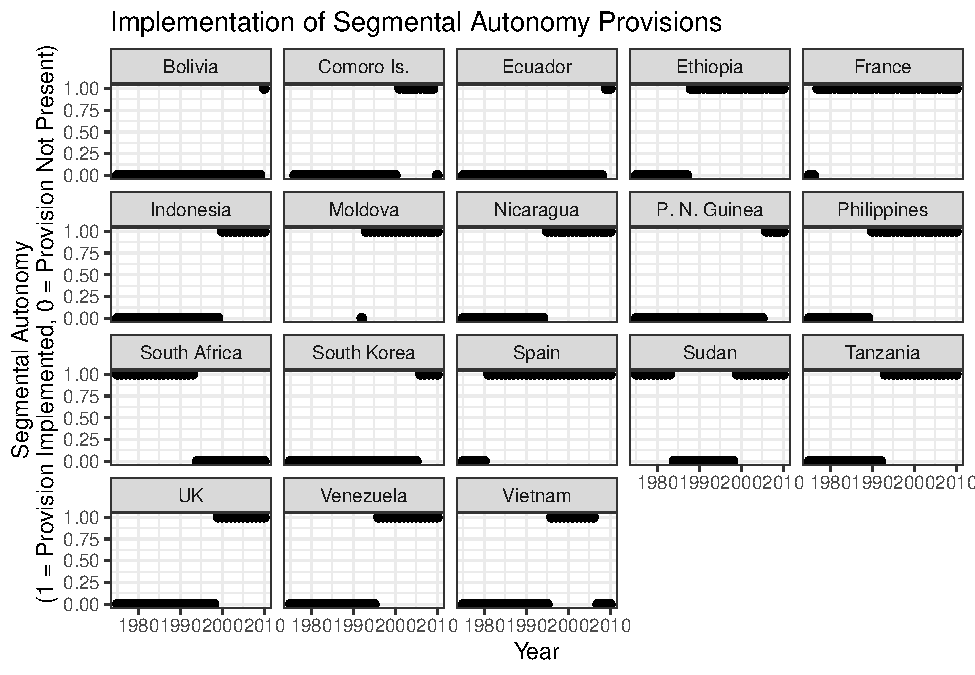
\includegraphics{02_tjbrailey_var_explore_files/figure-latex/unnamed-chunk-4-1.pdf}

\begin{Shaded}
\begin{Highlighting}[]
\KeywordTok{ggsave}\NormalTok{(gp1, }\DataTypeTok{filename =} \KeywordTok{paste0}\NormalTok{(here}\OperatorTok{::}\KeywordTok{here}\NormalTok{(), }\StringTok{"/vis/seg_auton_implement.png"}\NormalTok{), }\DataTypeTok{units =} \StringTok{"in"}\NormalTok{,}
       \DataTypeTok{width =} \DecValTok{11}\NormalTok{, }\DataTypeTok{height =} \DecValTok{7}\NormalTok{)}
\end{Highlighting}
\end{Shaded}

\begin{Shaded}
\begin{Highlighting}[]
\CommentTok{# Subdivisions of segmental autonomy}
\NormalTok{subed <-}\StringTok{ }\NormalTok{psp }\OperatorTok
\StringTok{  }\NormalTok{dplyr}\OperatorTok{::}\KeywordTok{filter}\NormalTok{(idc_subed }\OperatorTok{==}\StringTok{ }\DecValTok{1}\NormalTok{) }\OperatorTok
\StringTok{  }\NormalTok{dplyr}\OperatorTok{::}\KeywordTok{distinct}\NormalTok{(country, year)}
\KeywordTok{unique}\NormalTok{(subed}\OperatorTok{$}\NormalTok{country)}
\end{Highlighting}
\end{Shaded}

\begin{verbatim}
##  [1] "Afghanistan"                  "Argentina"                   
##  [3] "Australia"                    "Austria"                     
##  [5] "Belgium"                      "Bhutan"                      
##  [7] "Bolivia"                      "Bosnia-Herz"                 
##  [9] "Botswana"                     "Brazil"                      
## [11] "Bulgaria"                     "Burundi"                     
## [13] "Cambodia"                     "Canada"                      
## [15] "Chile"                        "China"                       
## [17] "Colombia"                     "Croatia"                     
## [19] "Cuba"                         "Denmark"                     
## [21] "Finland"                      "France"                      
## [23] "FRG/Germany"                  "Georgia"                     
## [25] "German Democratic Republic"   "Haiti"                       
## [27] "India"                        "Iraq"                        
## [29] "Ireland"                      "Italy"                       
## [31] "Japan"                        "Kazakhstan"                  
## [33] "Latvia"                       "Macedonia"                   
## [35] "Malaysia"                     "Mexico"                      
## [37] "Mongolia"                     "Montenegro"                  
## [39] "P. N. Guinea"                 "Pakistan"                    
## [41] "Paraguay"                     "Peru"                        
## [43] "Philippines"                  "Poland"                      
## [45] "Russia"                       "Slovakia"                    
## [47] "South Africa"                 "South Korea"                 
## [49] "Spain"                        "Sri Lanka"                   
## [51] "Sudan"                        "Sweden"                      
## [53] "Switzerland"                  "Taiwan"                      
## [55] "Thailand"                     "UAE"                         
## [57] "Uganda"                       "UK"                          
## [59] "Ukraine"                      "USA"                         
## [61] "Venezuela"                    "Vietnam"                     
## [63] "W. Samoa"                     "Yugoslavia (FRY)"            
## [65] "Zaire (Democ Republic Congo)"
\end{verbatim}

\begin{Shaded}
\begin{Highlighting}[]
\NormalTok{subtax <-}\StringTok{ }\NormalTok{psp }\OperatorTok
\StringTok{  }\NormalTok{dplyr}\OperatorTok{::}\KeywordTok{filter}\NormalTok{(idc_subtax }\OperatorTok{==}\StringTok{ }\DecValTok{1}\NormalTok{) }\OperatorTok
\StringTok{  }\NormalTok{dplyr}\OperatorTok{::}\KeywordTok{distinct}\NormalTok{(country, year)}

\NormalTok{subpolice <-}\StringTok{ }\NormalTok{psp }\OperatorTok
\StringTok{  }\NormalTok{dplyr}\OperatorTok{::}\KeywordTok{filter}\NormalTok{(idc_subpolice }\OperatorTok{==}\StringTok{ }\DecValTok{1}\NormalTok{) }\OperatorTok
\StringTok{  }\NormalTok{dplyr}\OperatorTok{::}\KeywordTok{distinct}\NormalTok{(country, year)}

\NormalTok{fedunits <-}\StringTok{ }\NormalTok{psp }\OperatorTok
\StringTok{  }\NormalTok{dplyr}\OperatorTok{::}\KeywordTok{filter}\NormalTok{(idc_fedunits }\OperatorTok{==}\StringTok{ }\DecValTok{1}\NormalTok{) }\OperatorTok
\StringTok{  }\NormalTok{dplyr}\OperatorTok{::}\KeywordTok{distinct}\NormalTok{(country, year)}

\NormalTok{author <-}\StringTok{ }\NormalTok{psp }\OperatorTok
\StringTok{  }\NormalTok{dplyr}\OperatorTok{::}\KeywordTok{filter}\NormalTok{(dpi_author }\OperatorTok{==}\StringTok{ }\DecValTok{1}\NormalTok{) }\OperatorTok
\StringTok{  }\NormalTok{dplyr}\OperatorTok{::}\KeywordTok{distinct}\NormalTok{(country, year)}
\KeywordTok{unique}\NormalTok{(author}\OperatorTok{$}\NormalTok{country)}
\end{Highlighting}
\end{Shaded}

\begin{verbatim}
##  [1] "Argentina"        "Australia"        "Austria"          "Belgium"         
##  [5] "Benin"            "Bosnia-Herz"      "Botswana"         "Brazil"          
##  [9] "Canada"           "Colombia"         "Comoro Is."       "Czech Rep."      
## [13] "Ethiopia"         "Fiji"             "Finland"          "France"          
## [17] "FRG/Germany"      "India"            "Italy"            "Malaysia"        
## [21] "Mexico"           "Nepal"            "Philippines"      "Senegal"         
## [25] "Spain"            "Sudan"            "Sweden"           "Switzerland"     
## [29] "Trinidad-Tobago"  "UAE"              "USA"              "Venezuela"       
## [33] "Yugoslavia"       "Yugoslavia (FRY)"
\end{verbatim}

\hypertarget{subset-code}{%
\section{Subset code}\label{subset-code}}

\begin{Shaded}
\begin{Highlighting}[]
\CommentTok{# By states that exhibit change in the auton variable}
\NormalTok{aut_t <-}\StringTok{ }\NormalTok{psp }\OperatorTok
\StringTok{  }\NormalTok{dplyr}\OperatorTok{::}\KeywordTok{filter}\NormalTok{(idc_auton }\OperatorTok{==}\StringTok{ }\DecValTok{1}\NormalTok{) }\OperatorTok
\StringTok{  }\NormalTok{dplyr}\OperatorTok{::}\KeywordTok{distinct}\NormalTok{(country) }\OperatorTok
\StringTok{  }\NormalTok{dplyr}\OperatorTok{::}\KeywordTok{pull}\NormalTok{()}

\NormalTok{aut_f <-}\StringTok{ }\NormalTok{psp }\OperatorTok
\StringTok{  }\NormalTok{dplyr}\OperatorTok{::}\KeywordTok{filter}\NormalTok{(idc_auton }\OperatorTok{==}\StringTok{ }\DecValTok{0}\NormalTok{) }\OperatorTok
\StringTok{  }\NormalTok{dplyr}\OperatorTok{::}\KeywordTok{distinct}\NormalTok{(country) }\OperatorTok
\StringTok{  }\NormalTok{dplyr}\OperatorTok{::}\KeywordTok{pull}\NormalTok{()}

\NormalTok{aut_t <-}\StringTok{ }\NormalTok{dplyr}\OperatorTok{::}\KeywordTok{as_tibble}\NormalTok{(aut_t)}
\end{Highlighting}
\end{Shaded}

\begin{verbatim}
## Warning: Calling `as_tibble()` on a vector is discouraged, because the behavior is likely to change in the future. Use `tibble::enframe(name = NULL)` instead.
## This warning is displayed once per session.
\end{verbatim}

\begin{Shaded}
\begin{Highlighting}[]
\NormalTok{aut_f <-}\StringTok{ }\NormalTok{dplyr}\OperatorTok{::}\KeywordTok{as_tibble}\NormalTok{(aut_f)}

\NormalTok{country_aut <-}\StringTok{ }\NormalTok{aut_t }\OperatorTok
\StringTok{  }\NormalTok{dplyr}\OperatorTok{::}\KeywordTok{filter}\NormalTok{(value }\OperatorTok\StringTok{ }\KeywordTok{unique}\NormalTok{(aut_f}\OperatorTok{$}\NormalTok{value))}

\NormalTok{psp_aut_variation <-}\StringTok{ }\NormalTok{psp }\OperatorTok
\StringTok{  }\NormalTok{dplyr}\OperatorTok{::}\KeywordTok{filter}\NormalTok{(country }\OperatorTok\StringTok{ }\KeywordTok{c}\NormalTok{(country_aut}\OperatorTok{$}\NormalTok{value))}

\CommentTok{# By states that have never had autonomy}
\NormalTok{psp_no_aut <-}\StringTok{ }\NormalTok{psp }\OperatorTok
\StringTok{  }\NormalTok{dplyr}\OperatorTok{::}\KeywordTok{group_by}\NormalTok{(country) }\OperatorTok
\StringTok{  }\NormalTok{dplyr}\OperatorTok{::}\KeywordTok{mutate}\NormalTok{(}\DataTypeTok{no_aut =} \KeywordTok{sum}\NormalTok{(idc_auton, }\DataTypeTok{na.rm =} \OtherTok{TRUE}\NormalTok{)) }\OperatorTok
\StringTok{  }\NormalTok{dplyr}\OperatorTok{::}\KeywordTok{filter}\NormalTok{(}\KeywordTok{sum}\NormalTok{(no_aut) }\OperatorTok{!=}\StringTok{ }\DecValTok{0}\NormalTok{)}

\CommentTok{# By ethnic fractionalization index}
\KeywordTok{mean}\NormalTok{(psp}\OperatorTok{$}\NormalTok{qog_al_ethnic, }\DataTypeTok{na.rm =} \OtherTok{TRUE}\NormalTok{)}
\end{Highlighting}
\end{Shaded}

\begin{verbatim}
## [1] 0.4509707
\end{verbatim}

\begin{Shaded}
\begin{Highlighting}[]
\KeywordTok{median}\NormalTok{(psp}\OperatorTok{$}\NormalTok{qog_al_ethnic, }\DataTypeTok{na.rm =} \OtherTok{TRUE}\NormalTok{)}
\end{Highlighting}
\end{Shaded}

\begin{verbatim}
## [1] 0.4840572
\end{verbatim}

\begin{Shaded}
\begin{Highlighting}[]
\KeywordTok{quantile}\NormalTok{(psp}\OperatorTok{$}\NormalTok{qog_al_ethnic, }\FloatTok{.67}\NormalTok{, }\DataTypeTok{na.rm =} \OtherTok{TRUE}\NormalTok{)}
\end{Highlighting}
\end{Shaded}

\begin{verbatim}
##    67% 
## 0.6252
\end{verbatim}

\begin{Shaded}
\begin{Highlighting}[]
\CommentTok{# By auton and ethnic fractionalization}
\NormalTok{psp_no_aut_frac <-}\StringTok{ }\NormalTok{psp_no_aut }\OperatorTok
\StringTok{  }\NormalTok{dplyr}\OperatorTok{::}\KeywordTok{filter}\NormalTok{(qog_al_ethnic }\OperatorTok{>}\StringTok{ }\KeywordTok{median}\NormalTok{(psp}\OperatorTok{$}\NormalTok{qog_al_ethnic, }\DataTypeTok{na.rm =} \OtherTok{TRUE}\NormalTok{))}
\end{Highlighting}
\end{Shaded}

\end{document}
